\documentclass{article}
\usepackage[T1]{fontenc}
\usepackage[preprint,nonatbib]{neurips_2025}
\usepackage{graphicx,booktabs,amsmath,amssymb}
\usepackage[hidelinks]{hyperref}
\newcommand{\RawCount}{81,444}
\newcommand{\UniqueCount}{80,697}
\newcommand{\DuplicateCount}{747}
\newcommand{\StyleCount}{27}
\newcommand{\TrainCount}{64,615}
\newcommand{\ValCount}{7,965}
\newcommand{\TestCount}{8,117}
\newcommand{\EpochCount}{40}
\newcommand{\BatchSize}{128}
\newcommand{\LatentDim}{100}
\newcommand{\Width}{64}
\newcommand{\TrainingSeed}{285}
\newcommand{\RealSeed}{286}
\newcommand{\LatentSeed}{1286}
\newcommand{\GeneratorParameters}{3,576,704}
\newcommand{\DiscriminatorParameters}{2,765,568}
\newcommand{\BatchesPerEpoch}{504}
\newcommand{\WideMinutes}{6.44}
\newcommand{\ResizeMinutes}{10.76}
\newcommand{\EvaluationCount}{5,000}
\newcommand{\TestFidProb}{0.0750}
\newcommand{\TestRealIS}{7.522}
\newcommand{\TestReduction}{39.6}
\newcommand{\ValBaseFid}{112.81}
\newcommand{\ValBaseIS}{3.212}
\newcommand{\ValWideFid}{67.62}
\newcommand{\ValWideIS}{4.402}
\newcommand{\ValResizeFid}{75.77}
\newcommand{\ValResizeIS}{4.713}
\newcommand{\TestBaseFid}{111.84}
\newcommand{\TestBaseIS}{3.213}
\newcommand{\TestWideFid}{67.58}
\newcommand{\TestWideIS}{4.402}

\title{Generating WikiArt Paintings with a DCGAN}
\author{ECE 285 Homework 2\quad\href{https://github.com/Tobudase/ece285-hw2-wikiart-gan}{Code on GitHub}}
\begin{document}
\maketitle
\suppressfloats[t]
\begin{abstract}
We compare three GAN configurations for $64\times64$ WikiArt generation. The wider DCGAN achieves the lowest validation FID (\ValWideFid), held-out test FID of \TestWideFid, and Inception Score of \TestWideIS. Generated paintings show clearer coarse structure, but fine detail remains limited.
\end{abstract}

\section{Data and implementation}
The assigned WikiArt archive~\cite{kaggle} contains \RawCount{} images. We apply EXIF orientation, convert to RGB, center crop and resize bicubically to $64\times64$. Deduplication by exact processed pixels removes \DuplicateCount{} images, leaving \UniqueCount{} images across \StyleCount{} styles. A seeded content hash yields \TrainCount{} training, \ValCount{} validation and \TestCount{} test images. Training ignores style labels; exact processed duplicates cannot cross splits, though near duplicates and shared artists may remain.

Our DCGAN~\cite{dcgan} maps Gaussian noise through five $4\times4$ transposed convolutions ($512,256,128,64,3$ channels at width 64), with batch normalization/ReLU in hidden blocks and output Tanh. The discriminator uses strided convolutions ($64,128,256,512$ channels), LeakyReLU(0.2), batch normalization except in the first block, and a final logit. Inputs use $[-1,1]$; convolution weights use $\mathcal{N}(0,0.02^2)$. Each step alternates a real-plus-fake BCE discriminator update and a non-saturating generator update; fake images are detached for the former.

\begin{table}[h]
\centering
\caption{Configuration of the selected wider DCGAN.}
\small
\begin{tabular}{ll@{\qquad}ll}
\toprule
Setting & Value & Setting & Value\\
\midrule
Epochs / batch size & \EpochCount{} / \BatchSize & Latent / base width & \LatentDim{} / \Width\\
Adam learning rate & $2\times10^{-4}$ & Adam $(\beta_1,\beta_2)$ & $(0.5,0.999)$\\
Training seed & \TrainingSeed & Eval real / latent seeds & \RealSeed{} / \LatentSeed\\
Generator parameters & \GeneratorParameters & Discriminator parameters & \DiscriminatorParameters\\
\bottomrule
\end{tabular}
\end{table}

Both new models train from scratch on one A100 80\,GB (PyTorch 2.4.1, CUDA 12.1), with \BatchesPerEpoch{} full batches per epoch. Training takes \WideMinutes{} min for the wider DCGAN and \ResizeMinutes{} min for the variant, which uses nearest-neighbor resize plus convolution, spectral normalization on discriminator convolutions, and hinge losses.

\begin{figure}[!ht]
\centering
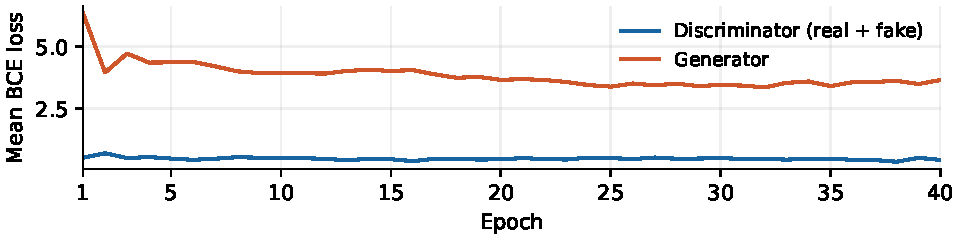
\includegraphics[width=.78\linewidth]{images/loss_curve.pdf}
\caption{Selected model's epoch-mean training losses. The discriminator curve sums real and fake BCE.}
\label{fig:loss}
\end{figure}

\newpage
\section{Evaluation and results}
For each evaluation, we generate \EvaluationCount{} images with noise seed \LatentSeed{} and sample \EvaluationCount{} real images without replacement (seed \RealSeed). Both use 8-bit RGB. Ignite computes the scores~\cite{ignite}. FID-2048 uses \texttt{pytorch-fid} pool3 features~\cite{fid}; FID-1000 uses ImageNet probabilities. Inception inputs are resized bilinearly to $299\times299$. IS is one aggregate, with no split-based deviation. All final checkpoints are compared on validation; the wider DCGAN is selected by lowest validation FID and then evaluated on test.

\begin{table}[h]
\centering
\caption{Final checkpoints. Lower FID-2048 and higher IS are preferable within this protocol.}
\small
\begin{tabular}{lrrrr}
\toprule
Model (width / epochs) & Val. FID & Val. IS & Test FID & Test IS\\
\midrule
Original DCGAN (32 / 20) & \ValBaseFid & \ValBaseIS & \TestBaseFid & \TestBaseIS\\
Wider DCGAN (64 / 40) & \textbf{\ValWideFid} & \ValWideIS & \textbf{\TestWideFid} & \textbf{\TestWideIS}\\
Resize + SN + hinge (64 / 40) & \ValResizeFid & \ValResizeIS & --- & ---\\
\bottomrule
\end{tabular}
\end{table}

The selected model lowers test FID by \TestReduction{}\% relative to the original. Its test FID-1000 is \TestFidProb; real-image test IS is \TestRealIS. Independent recomputation from saved features agrees with the metrics. Validation runs share CUDA; the original test result was computed on MPS with the same data and sampling protocol.

\begin{figure}[!ht]
\centering
\begin{minipage}{.32\linewidth}\centering
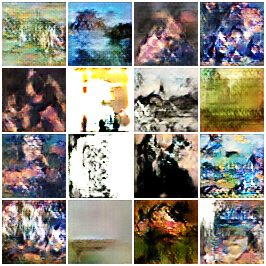
\includegraphics[width=\linewidth]{images/baseline.png}\\[-1pt]\small (a) Original DCGAN
\end{minipage}\hfill
\begin{minipage}{.32\linewidth}\centering
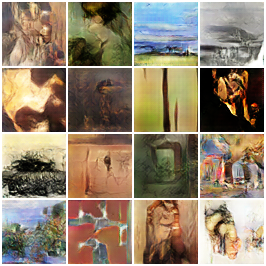
\includegraphics[width=\linewidth]{images/wide.png}\\[-1pt]\small (b) Wider DCGAN
\end{minipage}\hfill
\begin{minipage}{.32\linewidth}\centering
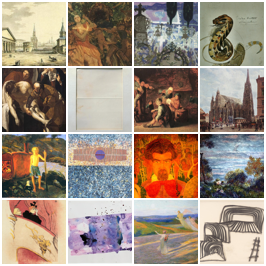
\includegraphics[width=\linewidth]{images/real.png}\\[-1pt]\small (c) Real test images
\end{minipage}
\caption{First 16 seeded samples per group. Both generators use the same latent sampling protocol.}
\end{figure}

\section{Discussion}
The wider DCGAN shows more coherent landscape layers and some recognizable figure outlines, but textures and small objects remain distorted. The resize/SN variant has higher validation IS yet worse FID than the wider DCGAN. Width and training duration change together relative to the original, so the gain cannot be attributed to either alone. One training seed, low resolution, and ImageNet features limit conclusions about variability and artistic fidelity.

{\small
\begin{thebibliography}{4}
\setlength{\itemsep}{0pt}
\bibitem{kaggle} Steubk. \href{https://www.kaggle.com/datasets/steubk/wikiart}{\emph{WikiArt}, Kaggle dataset, version 1}.
\bibitem{dcgan} A. Radford, L. Metz, and S. Chintala. Unsupervised representation learning with deep convolutional generative adversarial networks. ICLR, 2016.
\bibitem{ignite} PyTorch-Ignite. \href{https://pytorch-ignite.ai/blog/gan-evaluation-with-fid-and-is/}{GAN evaluation using FID and IS}.
\bibitem{fid} M. Heusel et al. GANs trained by a two time-scale update rule converge to a local Nash equilibrium. NeurIPS, 2017. Features: \href{https://github.com/mseitzer/pytorch-fid}{\texttt{pytorch-fid}}.
\end{thebibliography}
}
\end{document}
